
A system is scalable if it can easily adapt to 
increased (or reduced) demand. Scalablity
is usually limited by some sort of bottleneck.

\subsection{Parallelism programming}

\subsubsection{Vocabulary}
\begin{description}
    \item[Parallelism]: refers to techniques to make programs faster by
        performing several computations in parallel.

    \item[Concurrency]: is the composition of independently executing
        computations.

\end{description}

\subsubsection{Parallelization}
\begin{itemize}
    \item \textbf{Amdahl's law}:

        \begin{tabular}{m{0.5\linewidth}m{0.5\linewidth}}
            $$\quad S = \frac{1}{\alpha +
            \frac{1-\alpha}{N}}$$ where $\alpha$ is the sequential part and $N$ the
            number of cores.
            &
            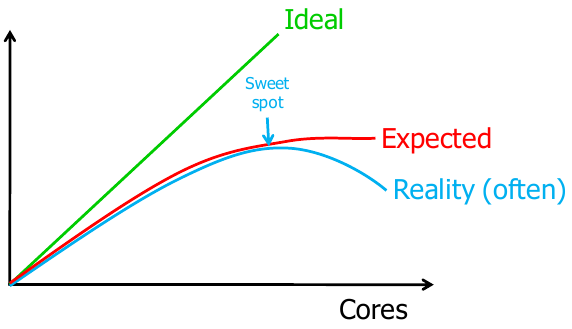
\includegraphics[width=6cm]{img/amdahl.png}
        \end{tabular}

        The coarse-grain (low rate communication) opposed to fine-grain (high rate) 
        parallelism is more efficient because it limits the communication and 
        coordination overheads by allow bigger task.

    \item \textbf{Dependencies}: Some task need to be after other which limits the degree of 
        parallelism. $\rightarrow$ Scheduling problem
\end{itemize}

\subsubsection{Synchronization}
Synchronization is needed when state is updated by different entities
(threads,process,servers,...)
\begin{description}
    \item[Race condition]: Result of the computation depends on the exact
        timing of the two threads of execution,i.e, the order in which instruction 
        are executed.

\end{description}

\subsubsection{Architecture}
\begin{itemize}
    \item Symmetric multiprocessing (SMP): all processors share same memory.

        \begin{tabular}{m{0.6\linewidth}m{0.3\linewidth}}
            \begin{itemize} 
                \item[+] Simplicity and easy to load balance 
                \item[-] Scalability limited and expensive
            \end{itemize}
            &
            \begin{tiny}
                \begin{tikzpicture}
                    \node[draw, rectangle] (1) {CPU};
                    \node[draw, rectangle] (2) [right=of 1] {CPU};
                    \node[draw, rectangle] (3) [right=of 2] {CPU};

                    \node[draw, rectangle] (11) [below=0cm of 1] {Cache};
                    \node[draw, rectangle] (21) [below=0cm of 2] {Cache};
                    \node[draw, rectangle] (31) [below=0cm of 3] {Cache};

                    \node (12) [below=0.3cm of 11] {};
                    \node (22) [below=0.3cm of 21] {};
                    \node (32) [below=0.3cm of 31] {};

                    \node (tmp) [below left= -0.2cm and 0.7cm of 12] {};
                    \node (tmp2) [below right=-0.2cm and 0.7cm of 32] {};

                    \draw (tmp) edge[double, <->] node[below](p) {Memory bus} (tmp2);
                    \draw (12) edge[<->] (11);
                    \draw (22) edge[<->] (21);
                    \draw (32) edge[<->] (31);

                    \node[draw, rectangle] (mem) [below=1.0cm of 21] {Memory};
                    \draw (mem) edge[<->] (p);
                \end{tikzpicture}
            \end{tiny}
        \end{tabular}

    \item Non Uniform memory architecture (NUMA)

        \begin{tabular}{m{0.6\linewidth}m{0.3\linewidth}}
            \begin{itemize} 
                \item[+] Better scalability and faster memory
                \item[-] Complicates programming and scalability limited
            \end{itemize}
            &
            \begin{tiny}
                \begin{tikzpicture}
                    \node[draw, rectangle] (1) {CPU};
                    \node[draw, rectangle] (2) [right=of 1] {CPU};
                    \node[draw, rectangle] (3) [right=of 2] {CPU};

                    \node[draw, rectangle] (11) [below=0cm of 1] {Cache};
                    \node[draw, rectangle] (21) [below=0cm of 2] {Cache};
                    \node[draw, rectangle] (31) [below=0cm of 3] {Cache};

                    \node[draw, rectangle] (12) [below=0.3cm of 11] {Memory};
                    \node[draw, rectangle] (22) [below=0.3cm of 21] {Memory};
                    \node[draw, rectangle] (32) [below=0.3cm of 31] {Memory};

                    \node (13) [below=0.3cm of 12] {};
                    \node (23) [below=0.3cm of 22] {};
                    \node (33) [below=0.3cm of 32] {};

                    \node (tmp) [below left= -0.2cm and 0.7cm of 13] {};
                    \node (tmp2) [below right=-0.2cm and 0.7cm of 33] {};

                    \draw (tmp) edge[double, <->] node[below](p) {Memory bus} (tmp2);
                    \draw (12) edge[<->] (11);
                    \draw (22) edge[<->] (21);
                    \draw (32) edge[<->] (31);

                    \draw (12) edge[<->] (13);
                    \draw (22) edge[<->] (23);
                    \draw (32) edge[<->] (33);
                \end{tikzpicture}
            \end{tiny}
        \end{tabular}

    \item Shared Nothing

        \begin{tabular}{m{0.6\linewidth}m{0.3\linewidth}}
            \begin{itemize} 
                \item[+] Nice scalability
                \item[-] Requires different programming model
            \end{itemize}
            &

            \begin{tiny}
                \begin{tikzpicture}
                    \node[draw, rectangle] (1) {CPU};
                    \node[draw, rectangle] (2) [right=of 1] {CPU};
                    \node[draw, rectangle] (3) [right=of 2] {CPU};

                    \node[draw, rectangle] (11) [below=0cm of 1] {Cache};
                    \node[draw, rectangle] (21) [below=0cm of 2] {Cache};
                    \node[draw, rectangle] (31) [below=0cm of 3] {Cache};

                    \node[draw, rectangle] (12) [below=0.3cm of 11] {Memory};
                    \node[draw, rectangle] (22) [below=0.3cm of 21] {Memory};
                    \node[draw, rectangle] (32) [below=0.3cm of 31] {Memory};

                    \node[draw, rectangle] (14) [below=0cm of 12] {Net card};
                    \node[draw, rectangle] (24) [below=0cm of 22] {Net card};
                    \node[draw, rectangle] (34) [below=0cm of 32] {Net card};

                    \node (13) [below=0.3cm of 14] {};
                    \node (23) [below=0.3cm of 24] {};
                    \node (33) [below=0.3cm of 34] {};

                    \node (tmp) [below left= -0.2cm and 0.7cm of 13] {};
                    \node (tmp2) [below right=-0.2cm and 0.7cm of 33] {};

                    \draw (tmp) edge[double, <->] node[below](p) {Network} (tmp2);
                    \draw (12) edge[<->] (11);
                    \draw (22) edge[<->] (21);
                    \draw (32) edge[<->] (31);

                    \draw (13) edge[<->] (14);
                    \draw (23) edge[<->] (24);
                    \draw (33) edge[<->] (34);
                \end{tikzpicture}
            \end{tiny}
        \end{tabular}

\end{itemize}


\subsection{Distributed programming}

\subsubsection{Vocabulary}
\begin{description}
    \item[Faults]: Some component is not working correctly
    \item[Failure]: System as a whole is not working correctly
\end{description}

\subsubsection{Wide-area network}
The transfert speed for some data are defined by some attributs:
\begin{enumerate}
    \item Propagation delay
    \item Bottlenecks capacity on the path
    \item Queueing delay, loss, reordering, congestion, rtt 
        (take in account by TCP)
\end{enumerate}

$\rightarrow$ wide-area networks complicates the communication and faults are
more common

\subsubsection{Faults}

Fault are a common event in distributed system and some faults
are correlated.

\begin{itemize}
    \item \textbf{Crash faults}: node simply stop
    \item \textbf{Rational behavior}: owner manipulates node to increase profit
        (ex: lies on the routes to have traffic through it's own AS)
    \item \textbf{Byzantine faults}: faulty node could do anything (ex: stop, send spam,
        attack other, tell lies,...)
\end{itemize}

To prevent fault, we can \textit{prevent} them by using verification,
\textit{detect} them or \textit{mask} them by using replicas. The problem of
using \textbf{replicas} is to be able to maintain consistency between them!

\subsubsection{Consistency}

\begin{itemize}
    \item \textbf{Strong consistency}: After update completes, all subsequent
        accesses will return the updated value

    \item \textbf{Weak consistency}: After update completes, accesses do not
        necessarily return the updated value;; some condition must be satisfied
        first (such as update needs to reach all the replicas)

    \item \textbf{Eventual consistency}: Specific form of weak consistency: If no
        more updates are made to an object, then eventually all reads will return
        the latest value

    \item \textbf{Causal consistency}: If client A has communicated to client B that it
        has updated a data item, a subsequent access by B will return the updated
        value, and a write is guaranteed to supersede the earlier write. Client C
        that has no causal relationship to client A is subject to the normal
        eventual consistency rules

    \item \textbf{Read-your-writes consistency}: Client A, after it has updated a data
        item, always accesses the updated value and will never see an older
        value.

    \item \textbf{Session consistency}: Like previous case but in the context of a
        session, for as long as the sessions remains alive.

    \item \textbf{Monotonic read consistency}: If client A has has seen a particular value
        for the object, any subsequent accesses will never return any previous
        values

    \item \textbf{Monotonic write consistency}: In this case the system guarantees to
        serialize the writes by the same process
\end{itemize}

We can combine them, and monotonic reads + read-your-write are most desirable
than eventual consistency.

\paragraph{Storage system consistency: example}

We have N nodes that can store data.
To write a value: Pick W replicas and write the value to each, using a fresh timestamp
To read a value:
\begin{itemize}
    \item Pick R replicas and read the value from each
    \item Return the value with the highest timestamp
    \item If any replicas had a lower timestamp, send them the newer value
\end{itemize}

\begin{tabular}{m{4cm}m{10cm}}
    Strong consistency :&
\begin{description}
    \item[Majority quorum] Always write to and read from a majority of nodes. At least one node knows the most recent value. tolerate up to ⌈N/2⌉ - 1 crashes. But have to read/write ⌊N/2⌋ + 1 values.
    \item[Read/write quorums] Read R nodes, write W nodes, s.t. R + W > N. Adjust performance of reads/writes. But availability can suffer.

        \begin{tabular}{m{3cm}m{12cm}}
            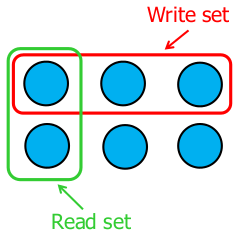
\includegraphics[width=3cm]{img/replicas} &
            
\includegraphics[width=7cm]{img/replicas2}
            \begin{itemize}
                \item[$\rightarrow$] Strong consistency
            \end{itemize} \\
        \end{tabular}
    \item[Consensus solutions] Paxos (for crash faults), PBFT (for Byzantine faults). Idea : Correct replicas ``outvote'' faulty ones.
\end{description}
\end{tabular}


The cap theorem : We can get at most two out of the three
\begin{itemize}
    \item Consistency : All clients single up-to-data copy of the data, even in the presence of concurrent updates
    \item Availability: Every request (including updates) received by a non-failing node in the system must result in a response, even when faults occur
    \item Partition-tolerance: Consistency and availability hold even when the network partitions
\end{itemize}

Dealing with network partitions when a partition is cut : Enter an explicit partition mode that can limit some operations.


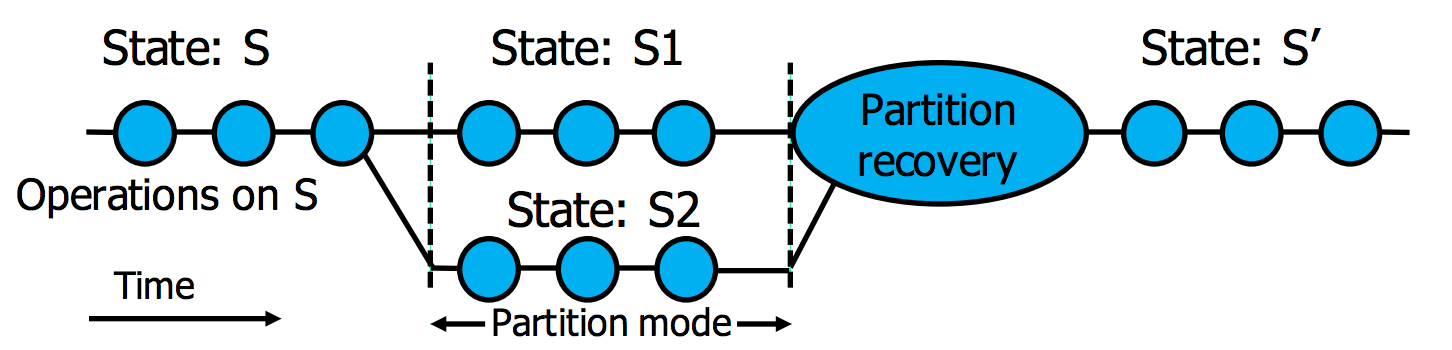
\includegraphics[width=\linewidth]{img/part}




\paragraph{Consensus}
\begin{enumerate}
    \item Clients send requests to each of the replicas
    \item Replicas coordinate and each return a result
    \item Client chooses one of the results, e.g., the one that is 
        returned by the largest number of replicas
    \item If a small fraction of the replicas returns the wrong result, or 
        no result at all, they are 'outvoted' by the other replicas
\end{enumerate}


\subsubsection{CAP theorem}
\begin{center}
    \begin{tikzpicture}
        \node (A) {\textcolor{red}{A}};
        \node (C) [below left= 2.5cm and 1.5cm of A] {\textcolor{red}{C}};
        \node (P) [below right= 2.5cm and 1.5cm of A] {\textcolor{red}{P}};

        \node[right =1cm of A, text width=4cm] {\scriptsize \textbf{Availability}: Each client can always read
        and write despite node failures};

        \node[left =1cm of C, text width=4cm] {\scriptsize \textbf{Consistency}: all clients always have the
        same view of the data at the same time};

        \node[right =1cm of P, text width=4cm] {\scriptsize \textbf{Partition-tolerance}: the
        system continues to operate despite arbitrary message loss};

        \draw (A) edge[-] node[left] {C\&A} (C);
        \draw (A) edge[-] node[right] {A\&P \tiny (Many replicas + relaxed consistency)} (P);
    \draw (C) edge[-] node[below] {\begin{tabular}{c}C\&P\\ \tiny (Many replicas + consensus) \end{tabular}} (P);
    \end{tikzpicture}
\end{center}


\paragraph{Actually}, we have a lot of partition and we have a trade-off
between C and A. \textbf{ACID} (atomicity, consistency, isolation, durability)
become \textbf{BASE} (basically available, soft-state, eventually consistent).


\subsection{Structure}
\begin{figure}[!h]
    \centering
    \begin{tikzpicture}

        \node[draw, rectangle, minimum height= 2cm] (L) {\rotatebox{90}{Load balancer}};
        \node[draw, rectangle, fill=black!40, minimum height= 2cm, text width=1cm, right= of L] (W) {};
        \node[draw, rectangle, fill= white, minimum height= 0.5cm, text width=1cm, below=-1cm of W] (W1) {};
        \node[above=0cm of W] (1) {Web server};

        \node[draw, rectangle, fill=black!40, minimum height= 2cm, text width=1cm, right= of W] (A) {};
        \node[draw, rectangle, fill=white, minimum height= 0.5cm, text width=1cm, below=-1cm of A] (A1) {};
        \node[above=0cm of A] (1) {App server};

        \node[draw, rectangle, minimum height= 2cm, right= of A] (C) {\rotatebox{90}{Caching}};
        \node[draw, rectangle, minimum height= 2cm, right= of C] (D) {Data store};

        \draw[->] (-2, 0) -- (L);
        \draw[->] (-2, -1) -- (L);
        \draw[->] (-2, 1) -- (L);

        \node[left=2cm of L] (R) {\rotatebox{90}{Request}};

    \end{tikzpicture}
    \caption{Cloud structure with 
        caching which is central to responsiveness. Cached data are used by the inner
    services to shield them form online load}
\end{figure}

\begin{itemize}
    \item \textbf{Stateless server}: Views a client request as an independent 
        transaction and responds to it


        Easy to scale and more robust because instance failure does not require
        overheas restoring state

    \item \textbf{Statefull server}: Scaling is challenging because we need to maintains 
        the state.

        \paragraph{Traditionnal approach is replication}:

        \begin{tabular}{m{12cm}m{5cm}}
            \begin{itemize}
                \item Data is written to a \textit{master server} and then
                    replicated to one or more \textit{slave servers}
                    (synchronously or asynchronously)
                \item Read operations can be handled by the slaves
            \end{itemize}
            But in this case, master becomes the write bottleneck and single point of failure.
            &
            \centering
            \begin{tikzpicture}
                \node[draw, rectangle] (M) {Master};
                \node[draw, rectangle, below=1cm of M] (S) {Slave};
                \node (I) [right= of M] {};
                \node (O) [right= of S] {};

                \draw[->, double] (I) edge node[above] {in/out} (M);
                \draw[<-, double] (I) edge (M);
                \draw[<-, double] (O) edge node[below] {out}(S);
                \draw[->, double] (M) edge (S);
            \end{tikzpicture}
        \end{tabular}


        \paragraph{Sharding with partitionning}
        The idea is to split data between multiple 
        machines and have a way to make sure that
        the data is available on the right place.
        Typically, define a \textbf{sharding key} and create a \textbf{shard mapping}.

        \begin{tabular}{cm{10cm}}
            This allow to have &
            \begin{itemize}
                \item a really high availability
                \item increase read and write throughput
                \item the possibility 
                    of doing more work in parallel within the application server.
                \item[But] the challenge is to find a good partitionning scheme.
            \end{itemize}
        \end{tabular}

        \textbf{Sharding} is not only for partitioning data 
        within a database, but can also be use to partition data across caching 
        servers (memcached, redis).
\end{itemize}

\paragraph{First-tier parallelism}
Parallelism is vital for fast interactive services, and 
parallel actions must focus on the \textbf{critical path}. This is the
contributor delay for the response delay and do
not care about asynchronous that are shortly.

\begin{center}
    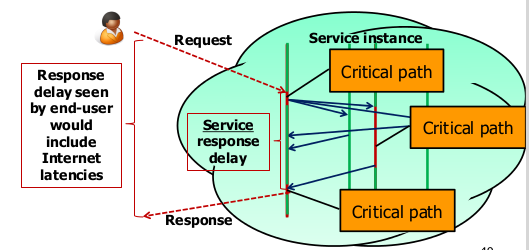
\includegraphics[width=9cm]{img/critical}
\end{center}


Note that update for replicas are typically done in asynchronous way, so we
might not experience much delay on the critical path.

$\rightarrow$ Asynchronous operations decouple systems and 
enable quicker responses at the expense strong 
consistency.
Indeed, this can rise some issues which result in inconsistency:
\begin{itemize}
    \item We don't know in which order replicas applying the update
    \item The leader can crash before replicas change and lose some
        update
\end{itemize}



